\documentclass[options]{article}
\usepackage{graphicx}
\graphicspath{{image/}}

\begin{document}
\title{A REPORT ON THE TRAFFIC JAM AROUND MAKERERE UNIVERSITY HILL}
\author{BARIYO DERRICK
15/U/4401/EVE
215008105}
\date{17/05/2017}
\maketitle

\section{\textbf{Terms of Reference}}
A report written in fulfilment of the need to be informed about the current jam situation of the roads around the Makerere hill.

\section{\textbf{Summary}} 
It’s the current jam situation of the roads around the Makerere hill that people would much be interested in but they can’t tell until they get to the road. The main aim of the report is to identify the roads that normally have jam and at what time of the day.
It was observed that each road has a different timing at which the jam normally occurs. A little more observation is required to get the best records over a goo period of time.


\section{\textbf{Introduction}} 
The jam along the roads around Makerere hill is caused because of many different reasons. The roads around Makerere hill include Sir Apollo Kagwa, Makerere hill, Kadaffi, Bombo.
The main aim of the report is to identify the time patterns and intervals of the jam on these different roads and letting people know of what time is conducive to use the different roads.


\section{\textbf{Body}} 
There are different factors that cause jam on these roads as i have listed below.
 \subsection{\textbf{Here are Some of the factors that course the jam:}}  

\begin{enumerate}
\item The day of the week because usually the working days have more jam on these roads compared to the weekends.
\item The time of the day, this is because morning hours between 07:00hrs - 09:00hrs and evening 18:00-21:00hrs   usually have more jam compared to the other hours of the day.
\item The constructions on some of these roads also bring about the jam.
\end{enumerate}


The limitations are that the jam occurrences on the different roads do not have a constant pattern of occurrence hence limiting the purpose of the report.
The jam can how ever be overcome by using alternate routes to one’s destination or opting for a road that as no or less jam.
Results from some of the records collected 


Table on the jam occurrence on the different roads on week days

\begin{tabular}{|l|l|l|l|l|}
\hline
Road& Sir Apollo Kagwa & Makerere hill & Kadaffi & Bombo \\
\hline
Time (hrs.) &  & & & \\
\hline
07:00-09:00& MEDIUM &HIGH&HIGH&HIGH \\
\hline
12:00-16:00 &FREE  & LOW&LOW & LOW\\
\hline
18:00-2100&HIGH  &MEDIUM & HIGH& HIGH\\
\hline

\end{tabular}
  
images of the statistics 

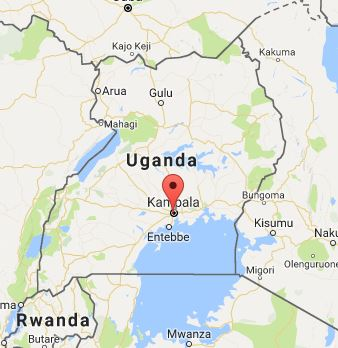
\includegraphics[width =6cm,height=4cm]{Captuhhre.JPG}
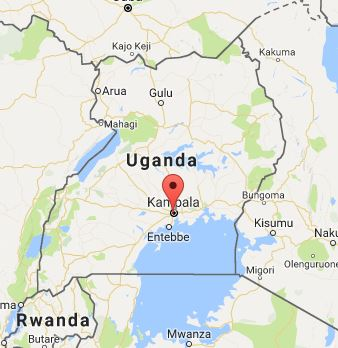
\includegraphics[width =6cm,height=4cm]{Captuhhre.JPG}

Screen shots of the application used.

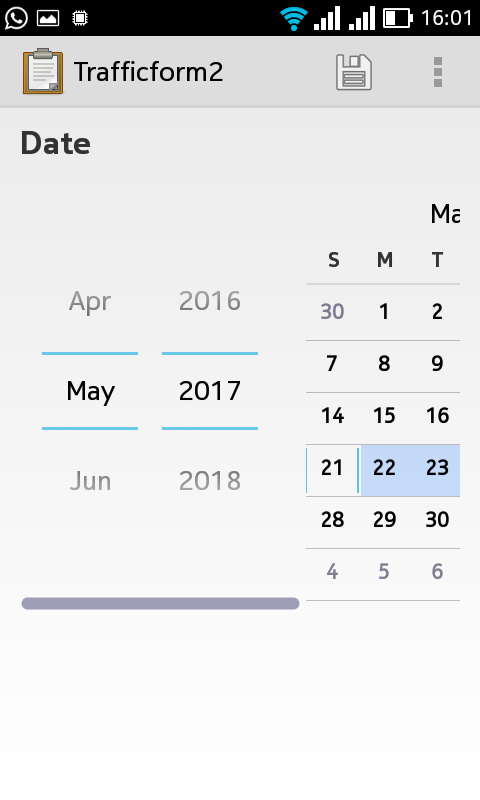
\includegraphics[width =3cm,height=4cm]{1.png}

\includegraphics[width =3cm,height=4cm]{2.png}
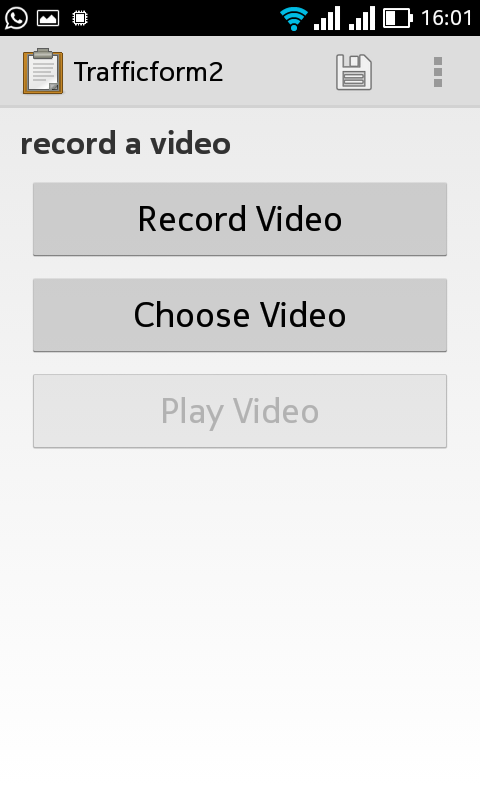
\includegraphics[width =3cm,height=4cm]{3.png}
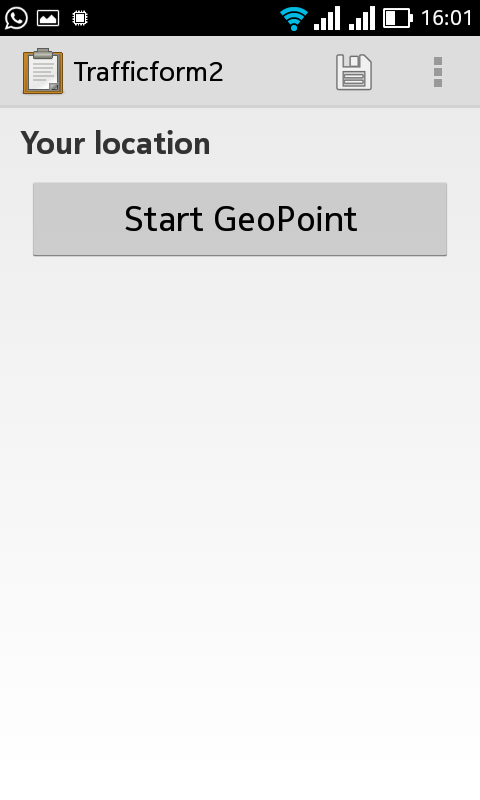
\includegraphics[width =3cm,height=4cm]{4.png}


\section{\textbf{Conclusion }} 
In conclusion a person should use a route according to day and time on which one is driving using any of the listed roads to prevent from being inconvenience of waiting in jam for long hours.
\end{document}